\documentclass[11pt]{article}

% set these commands
\newcommand{\course}{CSCI 534}
\newcommand{\proj}{Homework 06}
\newcommand{\dueDate}{2021-04-22}
\newcommand{\instructor}{David L. Millman}

\usepackage{../macros}

\newcommand{\A}{{\mathcal{A}}}

\begin{document}


\coverpage{06}


\vspace{1em}

This homework assignment occurs at the same time as the course project.  These
questions should take substantially less time then the first five assignments.
While I invite you to spend as much time on these problems as you like, I do not
expect you to spend any more than 3 hours on the entire assignment so that you
can focus on your projects.


\newpage
\section*{Problem 1}

We saw in class that the Voronoi diagram of a set of points in $\R^2$ is the
projection of the upper envelope of the dual lifted set of planes in $\R^3$.
What does the projection of the lower envelope correspond to? Similarly, what
does the projection of the upper convex hull of the points lifted to $\R^3$
correspond to?

You MAY (but do not need to) answer these questions by researching on the
internet. Cite the sources you were using and give an explanation in your own
words. \\

\answer
Let $P \subset \R ^2$ be our set of points.
For the first question, we want to know what happens when we project the lower envelope of the planes tangent to the lifted points.
We thought about this and came to the conjecture that the projection is the voronoi diagram of the vertices on the boundary of the convex hull of $P$.
The reason we think this is that points on the convex hull of will have tangent planes with the ``extreme'' normal vectors.
What we mean by this is that they have the normal vectors closest to vertical and closest to flat.
This means they will end up on the lower envelope at some region of the plane, although there is some weird flipping going on that we can't quite grasp.

Analogously, we think that the project of the upper convex hull is the delauney triangulation of the vertices on the boundary of the convex hull of $P$.
We think this because of an example we worked with where points are contained in the square $[-1,1]^2 \subset \R ^2$.
This is definitely not a proof but our guess worked nicely in the example!

\newpage
\section*{Problem 2}

We saw in class how to solve motion planning problems in $\R^2$ in a static
environment of polygonal obstacles by computing the configuration space with
Minkowski sums.  While theoretically interesting, often, explicitly computing
the configuration space is too computationally intensive.  Describe another
method for performing motion planning.

You MAY (but do not need to) answer this question by researching on the
internet. Cite the sources you were using and give an explanation in your own
words. \\

\answer
Instead of computing the entire Minkowski sum of the input to arrive at the configuration space, we take a more heuristic approach.
Like the motion planning algorithm we learned about in class, we are given the input, the polygonal object, and the source/target positions.
Our first step is to try to go in a straight line from the source to the target.
Instead of just moving the point, we attempt to move the boundary of the object (these are the green lines in Figure \ref{fig:motion}).
If we can move directly towards the target, we do so.
Otherwise, we move to the border of the first obstacle blocking us and repeat.
Figure \ref{fig:motion} shows some of the steps of our algorithm running.
It succeeds in stage 4.

\begin{figure}[h]
	\centering
	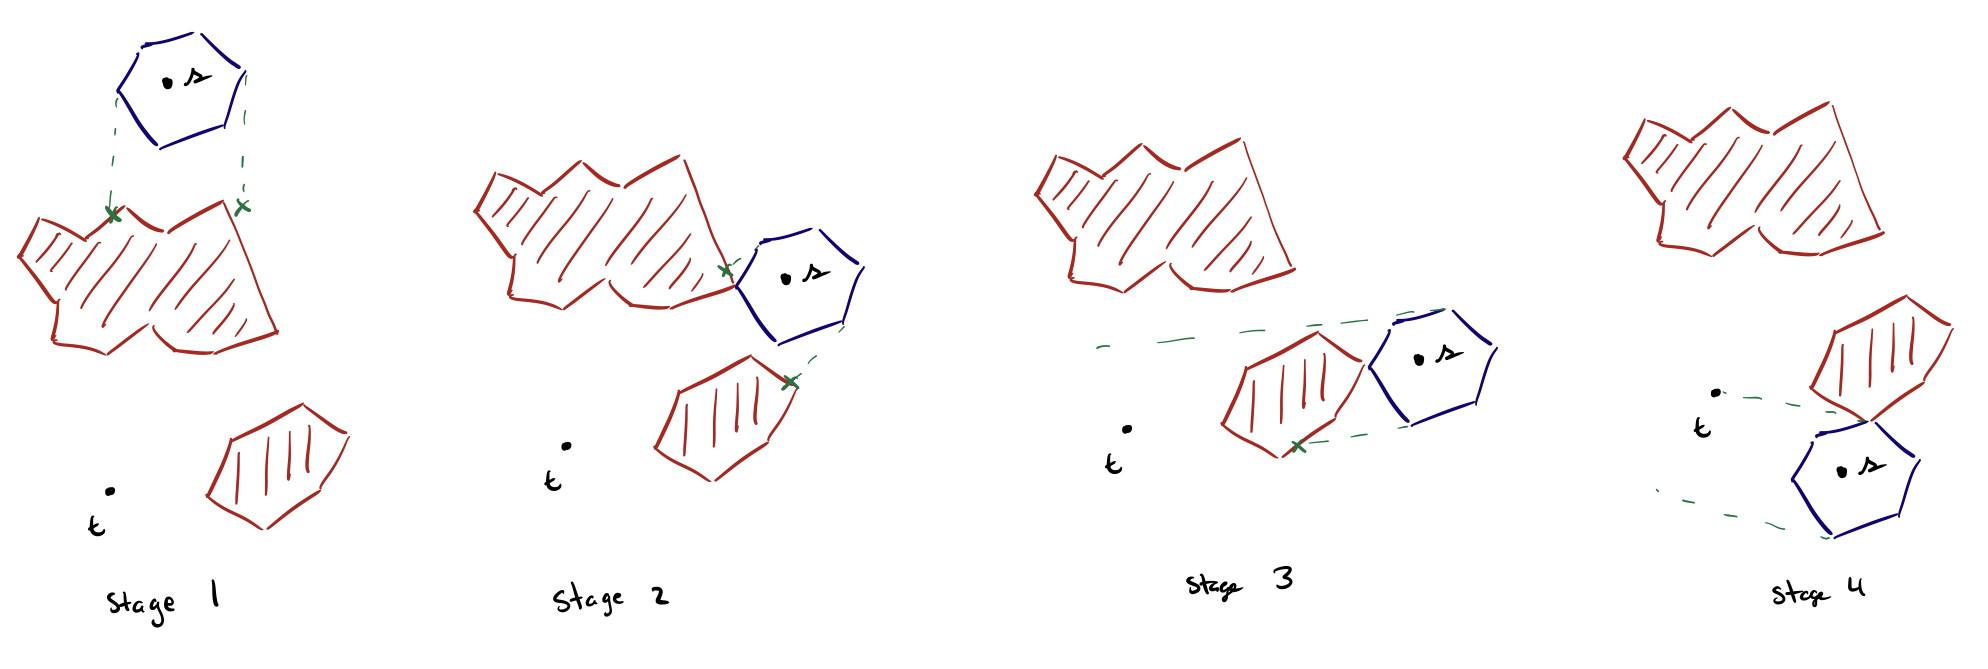
\includegraphics[width=0.9\textwidth]{motion-planning}
	\caption{A quick sketch of our idea in action}
	\label{fig:motion}
\end{figure}

\newpage
\section*{Problem 3}

Consider an arrangement $\A$ of six lines $\ell_1, \ell_2, \ldots, \ell_6$ and
let $f$ be an arbitrary vertex, edge, or face of $\A$. Then $f$ has an
associated sign vector $(s_1, s_2, s_3, s_4, s_5, s_6)$, where for each $1 \le i
\le 6$:

$$
    s_i =
    \begin{cases}
        +1, & \text{if $f$ lies above $l_i$} \\
        0,  & \text{if $f$ lies on $l_i$} \\
        -1, & \text{if $f$ lies below $l_i$}
    \end{cases}
$$

\begin{enumerate}

    \item For each of the sign vectors below, give an arrangement of six lines
        that has a vertex, edge, or face with this sign vector. Label the lines
        and mark the vertex, edge, or face. Make the arrangement simple, if
        possible, or argue why the arrangement cannot be simple.
        \begin{enumerate}
            \item $(+1, +1, +1, +1, +1, +1)$
            \item $(+1, 0, 0, -1, -1, -1)$
            \item $(-1, 0, 0, -1, +1, -1)$
            \item $(+1, -1, -1, -1, -1, -1)$
        \end{enumerate}

    \item Can one find a single arrangement of lines that contains a vertex,
        edge, or face for each of the four sign vectors? If you can, provide an
        example.  If you cannot, argue why not.

\end{enumerate}

\answer
\begin{enumerate}
	\item Figure \ref{fig:arrangments} the desired arrangements.
	They are all simple.
	For parts a and d, I chose a face and labeled it $F$.
	For parts b and c, I chose a vertex and labeled it $v$.

	\begin{figure}[h]
		\centering
		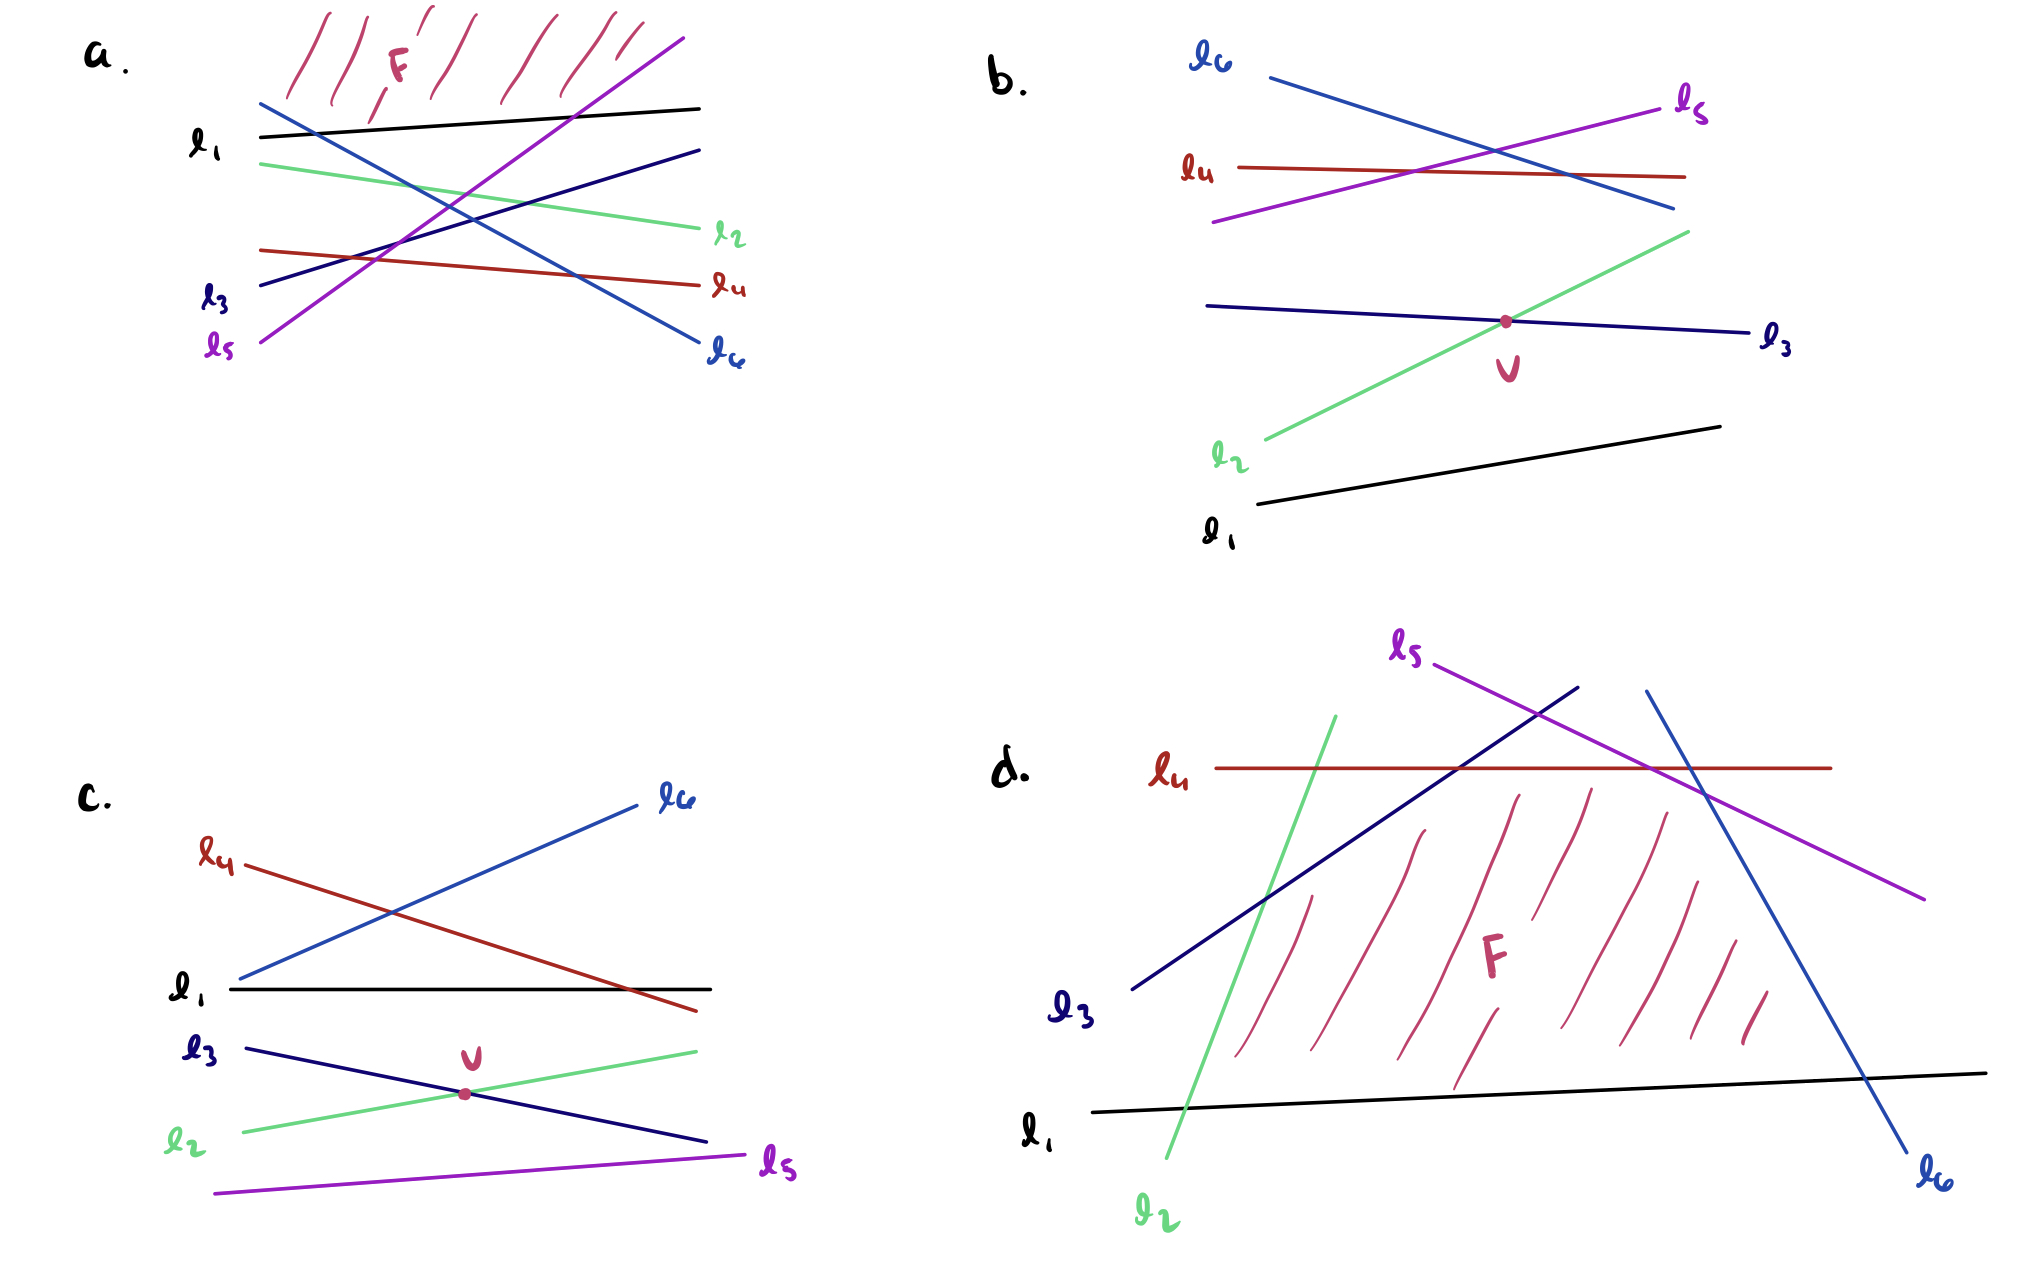
\includegraphics[width=0.9\textwidth]{arrangements}
		\label{fig:arrangments}
	\end{figure}

	\item We can't have an arrangement that contains a vertex, edge, or face for each of the sign vectors for the following reason.
	Parts b and c require that something (vertex, edge, or face) must lie precisely on both lines $l_2$ and $l_3$.
	The only object that can have this property is a vertex, label it $v$
	But then b and c have opposite requirements for $v$: b says $v$ must be above line $l_1$ while c says that $v$ must be below $l_1$.
	We cannot have a point both above and below a line so no arrangements exists that contains objects satisfying all four constraints.
\end{enumerate}

\newpage
\section*{Problem 4}

We saw in class a few applications of arrangements for solving geometric
problems. Find a problem whose solution was not described in class.  Give a
description of the problem and how one can use arrangements to solve the
problem.

You MAY (but do not need to) answer these questions by researching on the
internet. Cite the sources you were using and give an explanation in your own
words. \\

\answer
Suppose that you are given some set of lines in $\R ^2$ and you wish to compute the maximum finite area of the polygons formed by the lines.
One way to think of this (incidentally, it is how Elliott was struck with the idea) is to imagine that the lines are laser beams in a security system and we want to make sure that there is no ``face" large enough for someone to get through.

If we are given $n$ lines, we can compute the arrangement $O(n^2)$ time.
Then there are $O(n^2)$ convex faces.
For any convex shape, we can compute its area by picking a point in side the shape, forming triangles with the points on the boundary, and adding up the area of the triangles.
A strict bound on computing the area of any convex shape is $O(n)$.
But then a naive bound for computing the area of all of the faces would be $O(n^3)$ (this is $O(n)$ time for each of the $O(n^2)$ faces).
However, I feel like there is an argument similar to the zoning theorem where we can say that computing the area for all the faces ends up running in $O(n^2)$ time.
Then we can just pick the finite face with the largest area and we have our answer!

\end{document}
